\newpage
\section{Analiza problemu}		%2
\hspace{0.60cm}
Lista dwukierunkowa to lista, w której możemy poruszać się w dwóch kierunkach.
Każdy element zawiera co najmniej trzy pola: klucz, prev oraz next. W rezultacie
elementy wskazują zarówno swoje poprzedniki, jak i następniki. Strukturę logiczną listy przedstawiono na rysunku
\textbf{2.1}\footnote{Źródło: Contentplus.pl Sp. z o.o., licencja: CC BY-SA 3.0.}

\begin{figure}[!htb]
  \begin{center}
    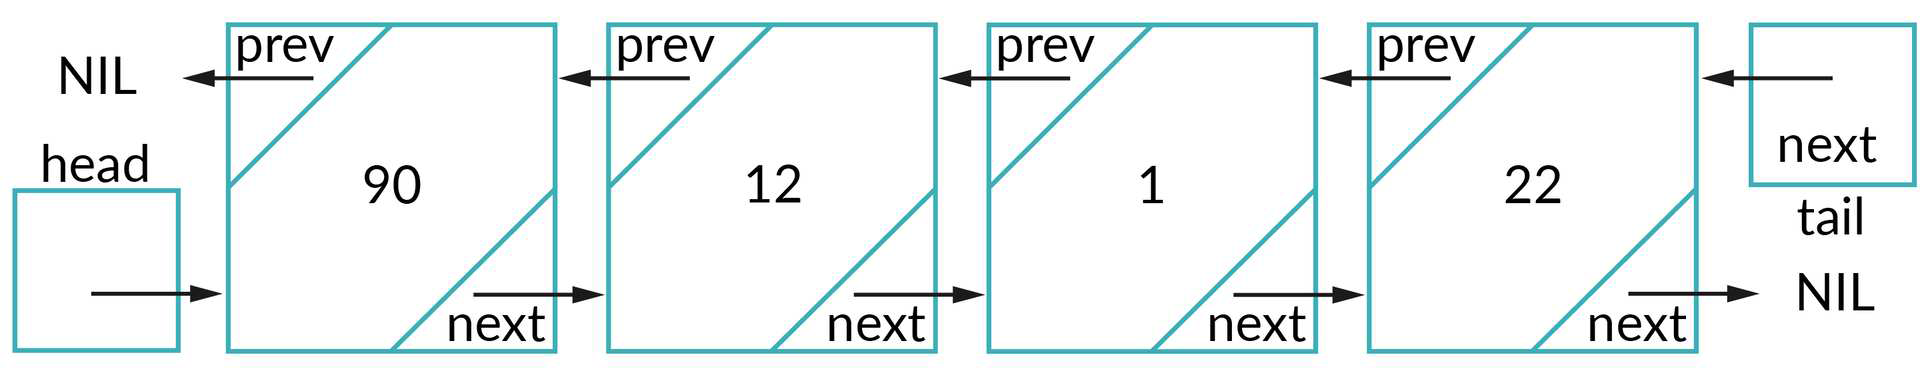
\includegraphics[width=\textwidth]{rys/lista-dwukierunkowa.png}
    \caption{Lista dwukierunkowa}\label{rys:lista_dwukierunkowa}
  \end{center}
\end{figure}

\subsection{Zastosowanie algorytmu listy dwukierunkowej\cite{ZPE}}

Listy dwukierunkowe są szeroko stosowane w różnych dziedzinach informatyki, gdy konieczne jest przechowywanie i manipulowanie dynamicznie zmieniającą się liczbą elementów, przy jednoczesnym zachowaniu możliwości poruszania się w obu kierunkach — do przodu i do tyłu. Typowe zastosowania list dwukierunkowych obejmują:

\begin{itemize}
  \item Implementację struktur takich jak deki (kolejki dwustronne), które pozwalają na dodawanie i usuwanie elementów z obu końców.
  \item Systemy zarządzania pamięcią, gdzie listy dwukierunkowe są używane do śledzenia dostępnych i zajętych bloków pamięci.
  \item Nawigację w przeglądarkach internetowych (przycisk „wstecz” i „dalej”), gdzie konieczne jest poruszanie się w obu kierunkach między odwiedzonymi stronami.
  \item Implementację buforów cyklicznych, gdzie struktura umożliwia płynne przechodzenie pomiędzy początkowym a końcowym elementem listy.
  \item Różne algorytmy wyszukiwania i sortowania, które wymagają przemieszczania się po danych w obu kierunkach.
\end{itemize}

\newpage
\subsection{Działanie listy dwukierunkowej}
\begin{itemize}
  \item \textbf{Wstawianie elementów} na początku, na końcu lub na podanym indeksie.

        Na rysunku \textbf{2.2}\footnote{Zdjęcie ze strony \url{https://www.programiz.com/dsa/doubly-linked-list}\cite{Programiz} \\ (Dostęp: 24.10.2024r.)} pokazano dodawanie elementu na początek listy.

        \begin{figure}[!htb]
          \begin{center}
            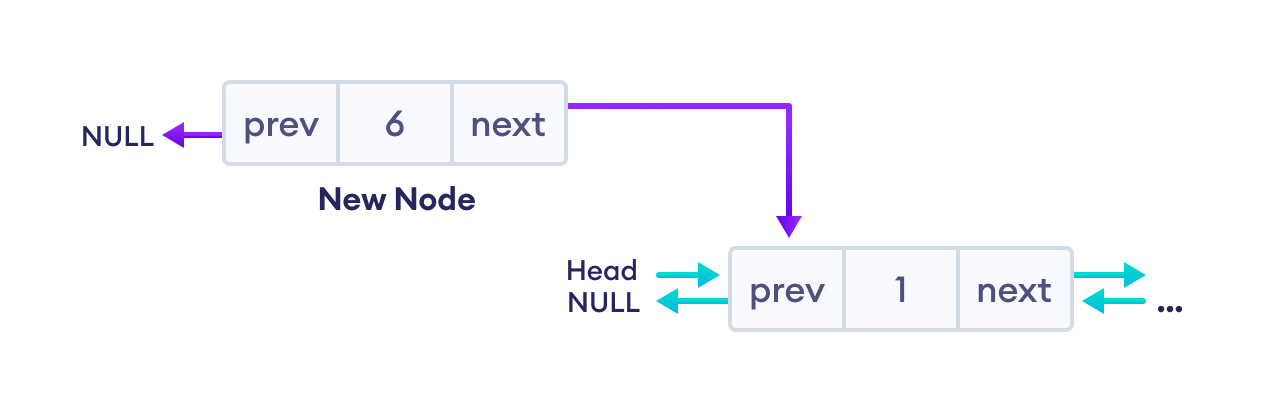
\includegraphics[width=\textwidth]{rys/dodawanie-elementu.png}
            \caption{Dodawanie elementu na początek listy}\label{rys:dodawanie_elementu}
          \end{center}
        \end{figure}

  \item \textbf{Usuwanie elementów} z początku, z końca lub z dowolnej pozycji w liście oraz czyszczenie listy.

        Na rysunku \textbf{2.3}\footnote{Zdjęcie ze strony \url{https://www.programiz.com/dsa/doubly-linked-list}\cite{Programiz} \\ (Dostęp: 24.10.2024r.)} pokazano usuwanie elementu z początku listy.

        \begin{figure}[!htb]
          \begin{center}
            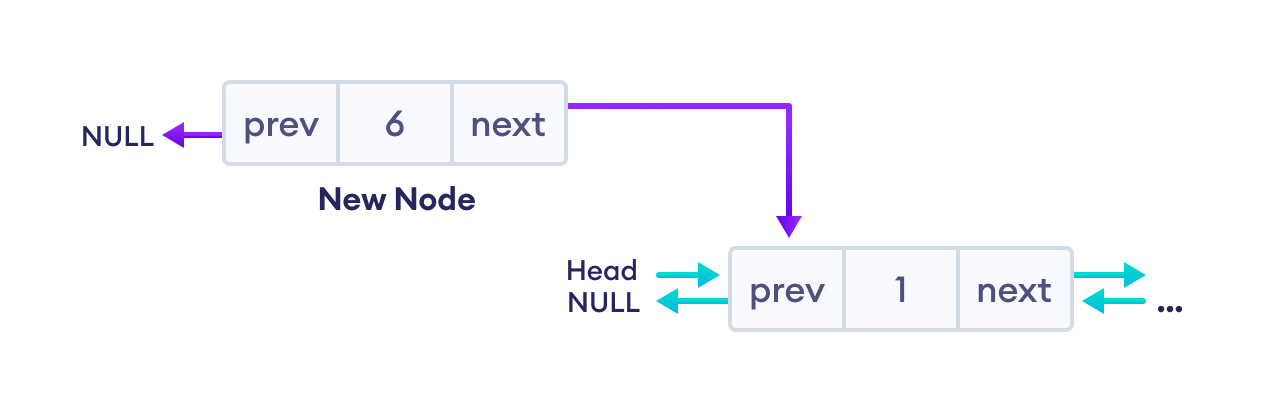
\includegraphics[width=\textwidth]{rys/dodawanie-elementu.png}
            \caption{Usuwanie elementu z początku listy}\label{rys:usuwanie_elementu}
          \end{center}
        \end{figure}

  \item \textbf{Wyświetlanie elementów} zarówno w kolejności od początku do końca, jak i w odwrotnej kolejności.

  \item \textbf{Przeglądanie listy}, zaczynając od określonego indeksu, w obu kierunkach (do przodu lub do tyłu).
\end{itemize}

\newpage

\subsection{Wykorzystanie systemu kontroli wersji Git i platformy GitHub}

\subsubsection[Systemy kontroli wersji]{Systemy kontroli wersji~\cite{ProGit}}

Czym są systemy kontroli wersji?
System kontroli wersji — oprogramowanie służące do śledzenia zmian głównie w kodzie źródłowym oraz pomocy programistom \\ w łączeniu zmian dokonanych w plikach przez wiele osób w różnym czasie.

Dlaczego warto znać systemy kontroli wersji
Proces tworzenia i rozwoju oprogramowania polega na nieustannym wprowadzaniu zmian w kodzie. Nawet jeśli pracujemy w pojedynkę z czasem zarządzanie takimi zmianami przy pomocy naiwnych metod (np. tworzenie nowego katalogu opisanego data i nazwą danej \\ wersji) staje się problematyczne, czasochłonne i na ogół nieefektywne. Nie mamy również łatwej możliwości archiwizacji czy cofania zmian. \\ Problem jest dodatkowo potęgowany kiedy mamy do czynienia z zespołem programistów pracującym nad projektem. Oprócz oczywistej konieczności ciągłego ręcznego przekazywania sobie zmian pojawia się kwestia rozwiązywania nieuniknionych konfliktów. \\ Wtedy właśnie z pomocą przychodzą systemy kontroli wersji.


\subsubsection[Czym jest Git]{Czym jest Git~\cite{ProGit}}
Git — system kontroli wersji utworzony w 2005 roku przez społeczność rozwijającą jądro systemu Linux (a w szczególności Linusa Torvaldsa, twórcę Linuksa)
po tym jak pogorszyły się jej relacje z firmą odpowiedzialną za stworzenie systemu kontroli BitKeeper, którego wówczas używali.
\\
Charakteryzują go przede wszystkim:
\begin{itemize}
  \item Szybkość
  \item Prosta konstrukcja
  \item Silne wsparcie dla nieliniowego rozwoju (tysięcy równoległych gałęzi)
  \item Pełne rozproszenie
  \item Wydajna obsługa dużych projektów, takich jak jądro systemu Linux (szybkość i rozmiar danych)
\end{itemize}

\subsubsection{Platformy hostowania kodu źródłowego}
Najpopularniejsze platformy do hostowania kodu to
\begin{itemize}
  \item \href{https://github.com/}{GitHub}
  \item \href{https://about.gitlab.com/}{GitLab}
  \item \href{https://bitbucket.org/product}{BitBucket}
  \item \href{https://sourceforge.net/}{SourceForge}
\end{itemize}

W tym przypadku skupimy się na platformie GitHub. Warto wspomnieć, że GitHub oferuje studentom darmową subskrypcję Pro do celów edukacyjnych jak również inne pakiety. Więcej na ten temat \href{https://education.github.com/students}{pod adresem}.
